\documentclass[12pt,a4paper]{article}
\usepackage[utf8]{inputenc}
\usepackage[russian]{babel}

\usepackage{fontspec}
\setmainfont[
	Ligatures=TeX,
	Extension=.otf,
	BoldFont=cmunbx,
	ItalicFont=cmunti,
	BoldItalicFont=cmunbi,
]{cmunrm}
\setsansfont{Arial}
\setmonofont{Consolas}
\RequirePackage{polyglossia}
\setdefaultlanguage{russian}
\setotherlanguage{english}

\textheight=24cm % высота текста
\textwidth=16cm % ширина текста
\oddsidemargin=0pt % отступ от левого края
\topmargin=-1.5cm % отступ от верхнего края
\parindent=24pt % абзацный отступ
\parskip=5pt % интервал между абзацами
\tolerance=2000 % терпимость к "жидким" строкам
\flushbottom % выравнивание высоты страниц
\usepackage{indentfirst}

\usepackage[fleqn]{amsmath}
\usepackage[T1]{fontenc}
\usepackage{mathtools}
\usepackage{color}
\usepackage{ulem}
\normalem
\makeatletter
\newenvironment{sqcases}{\matrix@check\sqcases\env@sqcases}{\endarray\right.}\def\env@sqcases{\let\@ifnextchar\new@ifnextchar\left\lbrack\def\arraystretch{1.2}\array{@{}l@{\quad}l@{}}}\makeatother

\title{Заметки по химии из старых школьных тетрадок.}
\author{Авторы: Я и школа.}
\date{Алматы, 2016}

\begin{document}

%--------------------------------------------------------------------------------%
%--------------------------------------------------------------------------------%

\maketitle

\tableofcontents

\thispagestyle{empty}

%--------------------------------------------------------------------------------%
%--------------------------------------------------------------------------------%

\newpage

\setcounter{page}{1} % начать нумерацию с номера 1

\section{8 класс}

\subsection{Определения}

{\bfseries Химия} --- наука о веществах, их свойствах превращениях веществ и явлениях сопровождающих эти превращения.

{\bfseries Свойствами вещества} называют признаки по которым вещества отличаются друг от друга, или сходны между собой.

{\bfseries Задачи химии} ---  изучение свойств веществ с целью дальнешйшего их применения, получения новых химических веществ, необходимых для нужд человека, рациональное использование природных ресурсов, охрана окружающей среды.

{\bfseries Атомы} --- сельчайшие химически неделимые частицы вещества.

{\bfseries Кристаллическая решетка} --- это предполагаемый каркас в узлах которого находятся атомы, молекулы или другие частицы.

{\bfseries Химический элемент} --- определенный вид атома.

{\bfseries Относительная атомная масса элемента} --- показывает, во сколько раз масса его атома больше $\frac{1}{12}$ массы атома углерода. Пишется как Ar(Э). Безразмерная величина.

{\bfseries Химическая формула} --- условная запись состава вещества посредством химических занков и индексов.

{\bfseries Валентность} --- свойство атомов химического элемента присоединять определенное число атомов других химических элементов.

{\bfseries Горением} называется реакция окисления вещества, т.е. взаимодействия с кислородом. При этой реакции характерно выделение тепла и света. При горении простых и сложных веществ образуются различные оксиды.

%--------------------------------------------------------------------------------%

\subsection{Деление веществ}

Вещества делятся на {\bfseries чистые} и {\bfseries смеси}.

{\bfseries Чистые вещества} состоят из частиц одного вида, обладают постоянными физическими свойствами. Так же чистые вещества обладают постоянными физическими свойствами. {\itshape Например}: медь, свинец, дистилированная вода.

{\bfseries Смеси} состоят из частиц разного вида, не обладают постоянными физическими свойствами. {\itshape Например}: молоко, газированная вода, воздух.

\medskip\hrule\medskip

Смеси делятся на {\bfseries однородные} и {\bfseries неоднородные}.

{\bfseries Однородными} называют такие смеси, в которых даже с помощью микроскопа нельзя обнаружить частицы веществ входящих в смесь. {\itshape Например}: раствор сахара, любые растворы.

{\bfseries Неоднородными} называют такие смеси в которые невооруженным глазом или при помоищ микроскопа можно заметить частицы веществ составляющих смсь. {\itshape Например}: молоко, газированная вода, глина с водой.

\medskip\hrule\medskip

Элементы делятся на {\bfseries металлы} и {\bfseries неметаллы}.

{\bfseries Металлы} обладают признаками: серебристо-серого цвета, металлический блеск; ковкость; имеют магнитные свойтсва;  высокие тепло-электро проводимости; свободные электроны. {\itshape Например:} железо, медь, титан.

{\bfseries Неметаллы} не имеют металлических свойств. {\itshape Например}: сера, углерод, водород.

Металлы начинаются во втором ряду с Лития, заканчиваются Бериллием, в последнем ряду начинаются с Франция, заканчиваются Астатом. В остальных рядах металлами считаются вещества, находищиеся под линие, проведенной из концов металлов первого и последнего ряда. Все остальное неметаллы. Так же последний столбик содержит инертные газы, они ни с чем не взаимодействуют.

%--------------------------------------------------------------------------------%

\subsection{Химические явления}

При {\bfseries химических реакциях} исходные вещества превращаются в другие вещества, обладающие другими свойствами. Об этом можно судить по {\itshape внешним признакам химических реакций}:

\begin{enumerate}
\item Выделение теплоты(иногда света).
\item Изменение окраски.
\item Появление запаха.
\item Образование осадка.
\item Выделение газа.
\end{enumerate}

{\itshape Условия возникновения химических реакций}:

\begin{enumerate}
\item Измельчение веществ.
\item Растворение веществ.
\item Доведение веществ до необходимой температуры.
\end{enumerate}

%--------------------------------------------------------------------------------%

\subsection{Типы реакций}

\begin{enumerate}
\item {\bfseries Реакцией соединения} называется такая реакция, в результате которой из двух или нескольких простых или сложных веществ образуется одно или более сложных веществ.
	$$\mathrm{ A + B \xrightarrow{} AB }$$
	$$\mathrm{ Fe + S \xrightarrow{} FeS }$$

\item {\bfseries Реакцией разложения} называется такая реакция, в результате которой из одного сложного вещества получается два или несколько простых или сложных веществ.
	$$\mathrm{ AB \xrightarrow{t^{\circ}} A + B }$$
	$$\mathrm{ 2Hg O \xrightarrow{t^{\circ}} 2Hg + O_2 }$$
	 
\item {\bfseries Реакцией замещения} называется реакция протекающая между простым и сложным веществами, при которой атомы простого вещества замещают атомы одного из элементов в сложном веществе.
	$$\mathrm{ AB + C \xrightarrow{} CB + A }$$
	$$\mathrm{ 2H Cl + Fe \xrightarrow{} Fe Cl_2 + H_2 }$$

\item {\bfseries Реакцией обмена} называется реакция между двумя сложными веществами в ходе которых они обмениваются составными частями.
	$$\mathrm{ AB + CD \xrightarrow{} CB + AD }$$
	$$\mathrm{ Ba Cl_2 + Na_2 S \xrightarrow{} Ba S + 2Na Cl }$$

\end{enumerate}

%--------------------------------------------------------------------------------%

\subsection{Типы реакций}

Реакции делятся на {\bfseries эндотермические}(эндо --- внутри) и {\bfseries экзотермические}(экзо --- наружу).

{\bfseries Эндотермическая} --- это такая реакция, в которая протекает с поглощением энергии.

{\bfseries Экзотермическая} --- это такая реакци, которая протекает с выделением теплоты.

Количество теплоты, которое выделяется или поглощается при химических реакциях называется {\bfseries тепловым эффектом реакции}.

Химическое уравнение, в котором указывается тепловой эффект называется {\bfseries термохимическим уравнением реакций}.
	$$\mathrm{ C + O_2 \xrightarrow{} C O_2 + 402,24\ \text{кДж} }$$
	
%--------------------------------------------------------------------------------%

\subsection{Газы}

{\bfseries Закон Авогадро}: в равных объемах различных газов при одинаковых условиях содержится одинаковое число молекул. {\itshape Следствие}: одинаковое количество газов при одинаковых условиях занимают одинаковый объем.

{\bfseries Молярный объем} --- показывает объем одного моль вещества при н.у, и он будет равен $ V_m = 22,4 \frac{\text{л}}{\text{моль}} $.

{\bfseries Относительная плотность газа} показывает во сколько раз один газ тяжелее другого. Обозначается как $ D_{\mathrm{H_2}}(\mathrm{O_2}) = \frac{Mr(\mathrm{O_2})}{Mr(\mathrm{H_2})} = \frac{32}{2} = 16 $.

$ Mr(\text{воздуха}) = 29 $.

$\displaystyle M_{\text{смеси}} = \frac{M_1\,\nu_1 + M_2\,\nu_2 + \dots}{\nu_1 + \nu_2 + \dots} $

%--------------------------------------------------------------------------------%

\subsection{Кислоты, оксиды, основания, соли}

{\bfseries Кислоты} --- сложные вещества состоящие из атомов водорода и кислотных остатков. {\itshape Например}: $\mathrm{ H Cl }$, $\mathrm{ H_2 S }$, $\mathrm{ H_2 PO_4 }$.

{\bfseries Оксиды} --- сложные вещества бинарные, один из атомов --- кислород. {\itshape Например}: $\mathrm{ Na_2 O }$, $\mathrm{ CaO }$.

\noindent\begin{tabular}[t]{||p{3.85cm}|p{3.4cm}|p{3.9cm}|p{3.2cm}||}
\hline
	Кислотные оксиды & Основные оксиды & Амфотерные оксиды & Безразличные оксиды \tabularnewline
\hline
	Оксиды неметаллов, при взаимодействии с водой образуется соответствующая кислота. Реакция не происходит для $\mathrm{Si O_2}$. {\itshape Например}: 
	
	$\mathrm{S O_2 \Rightarrow H_2 S O_4}$
	
	$\mathrm{C O_2 \Rightarrow H_2 C O_3}$ &
	Оксиды металлов. При взаимодействии с водой образуются основания(гидроксиды). {\itshape Например}: 
	
	$\mathrm{Na_2 O \Rightarrow 2Na O H}$
	
	$\mathrm{Ca O \Rightarrow Ca(O H)_2}$  &
	Оксиды обладают двойственными свойствами(кислотными и основными). Амфортерными свойствами обладают: $\mathrm{Be O}$, $\mathrm{Zn O}$, $\mathrm{Al_2 O_3}$, $\mathrm{Cr_2 O_3}$, $\mathrm{Mn O_2}$. {\itshape Например}: 
	
	$\mathrm{Zn O \Rightarrow Zn(O H)_2 }$ $\mathrm{\Rightarrow H_2 Zn O_2}$ &
	Оксиды, не соответсвующие ни кислотам, ни основаниям. {\itshape Например}: $\mathrm{N O}$, $\mathrm{N O_2}$, $\mathrm{N_2 O}$. \tabularnewline
\hline
\end{tabular}

{\bfseries Основания} --- сложные вещства, состоящие из атомов металлов, соединенных одной или несколькии гидроксо-группами. {\itshape Например}: $\mathrm{ NaOH }$, $\mathrm{ Ca(OH)_2 }$.

{\bfseries Соли} --- сложные вещества состоящие из атомов металлов и кислотных остатков.

\noindent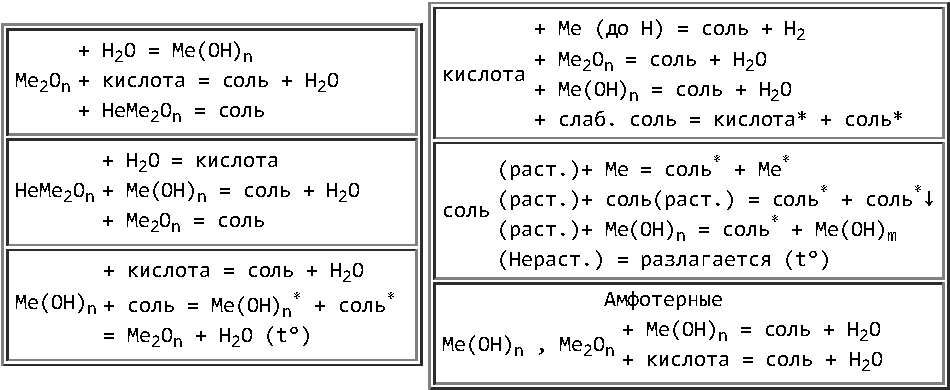
\includegraphics[width=1\textwidth]{ximiya-crop}

\subsection{Растворы}

{\bfseries Растворы} - однородные смеси, состоящие из молекул растворенного вещества и растворителя.

Растворы бывают {\bfseries насыщенные}, {\bfseries перенасыщенные} и {\bfseries ненасыщенные}.

{\bfseries Насыщенные растворы} --- такие растворы, в которыъ при данных условиях нельзя растворить вещества.

{\bfseries Перенасыщенные растворы} --- неоднородная смесь, которая состоит из насыщенного раствора и нерастворенного вещества.

{\bfseries Ненасыщенные растворы} --- это растворы, в которых еще можно растворить вещества при данных условиях.

\subsection{Электроотрицательность}

{\bfseries Электроотрицательность} --- свойство атомов притягивать к себе электроны.

Наименьшая электроотрицательность у цезия, наибольшая у фтора.

Чем больше отличается электроотрицательность элементов, тем прочнее химическое соединение.

{\bfseries Ковалентная связь} образуется между неметаллами.

{\bfseries Ионная связь} образуется между металлами и неметаллами.

{\bfseries Металлическая связь} образуется между одинаковыми металлами.

Положительные ионы --- {\bfseries катионы}. Отрицательные ионы --- {\bfseries анионы}.

\subsection{Заметки}

\begin{minipage}{0.4\textwidth}
	Названия соединений:
	
	\noindent\begin{tabular}[t]{|c|c|}
	\hline
	С чем & Название \tabularnewline
	\hline
	Кислород & Оксид \tabularnewline
	Водород & Гидрид \tabularnewline
	Углерод & Карбид \tabularnewline
	Хлор & Хлорид \tabularnewline
	Азот & Нитрид \tabularnewline
	Йод & Йодид \tabularnewline
	Сера & Сульфид \tabularnewline
	Фосфор & Фосфид \tabularnewline
	Бром & Бромид \tabularnewline
	Фтор & Фторид \tabularnewline
	\hline
	\end{tabular}
\end{minipage}
\hfill
\begin{minipage}{0.4\textwidth}
	Названия численных приставок:
	
	\noindent\begin{tabular}[t]{|c|c|}
	\hline
	Количество & Название \tabularnewline
	\hline
	1 & моно \tabularnewline
	2 & ди \tabularnewline
	3 & три \tabularnewline
	4 & тетра \tabularnewline
	5 & пента \tabularnewline
	6 & гекса \tabularnewline
	7 & гепта \tabularnewline
	8 & окта \tabularnewline
	9 & нона \tabularnewline
	10 & дека \tabularnewline
	\hline
	\end{tabular}
\end{minipage}

Все газообразные вещества в уравнениях реакции записываются в виде соединения газа с самим собой. {\itshape Например}: $\mathrm{O_2}$, $\mathrm{N_2}$, $\mathrm{H_2}$.

%--------------------------------------------------------------------------------%
%--------------------------------------------------------------------------------%

\end{document}